\documentclass[12pt]{book}
\usepackage[utf8]{inputenc}
\usepackage[margin=1.25in]{geometry}
\usepackage{graphicx}
\usepackage{amsmath , amssymb ,ragged2e}
\usepackage{bm}
\usepackage{esvect}
\usepackage{centernot}
\usepackage[usestackEOL]{stackengine}
\usepackage{eqparbox} 
\newcommand{\lagrange}{\mathcal{L}}
\newcommand{\fourier}{\mathcal{F}}
\newcommand{\x}{\chi}


\begin{document}
    \chapter{Phenomene de propagation unidimensionnels non dispersif}
        \subsubsection*{dispersif}
            milieu dans lequel les differents frequences constituant l'onde se propagent a des differantes vitesse  
        \section{Les ondes}
            \begin{itemize}
                \item C est une propagation d'une perturbation a motif unique ou a motif periodique
                \item c est un champ scalaire ou vectoriel ,definie dans un domaine de l espacec , dont les dependences spatiales et temporelles sont couplees par des equations aux derivees partielles apelees equation d onde
                    \begin{itemize}
                        \item un champ est une fonction qui depend de l abscisse x et du temps t , et qui decrit les propriete locales d'un milieu 
                        \item Champ scalair : a chaque point de lespace on associe un nombre (scalair)
                        \item Champ vectoriel : a chaque point de lespace on associe un vecteur 
                    \end{itemize}
                    \begin{center}
                        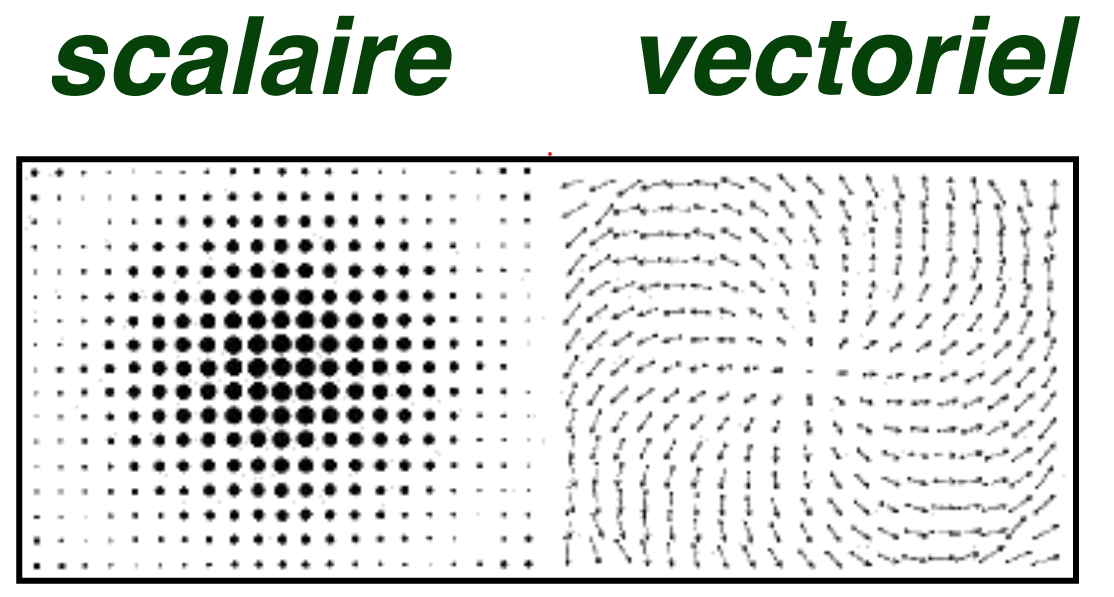
\includegraphics[width=0.4\linewidth]{pic/champscalairvectoriell.png}
                    \end{center}
            \end{itemize}
        \section{Classification des ondes }
            \begin{itemize}
                \item Ondes planes : front d'ondes sont des plans \\ 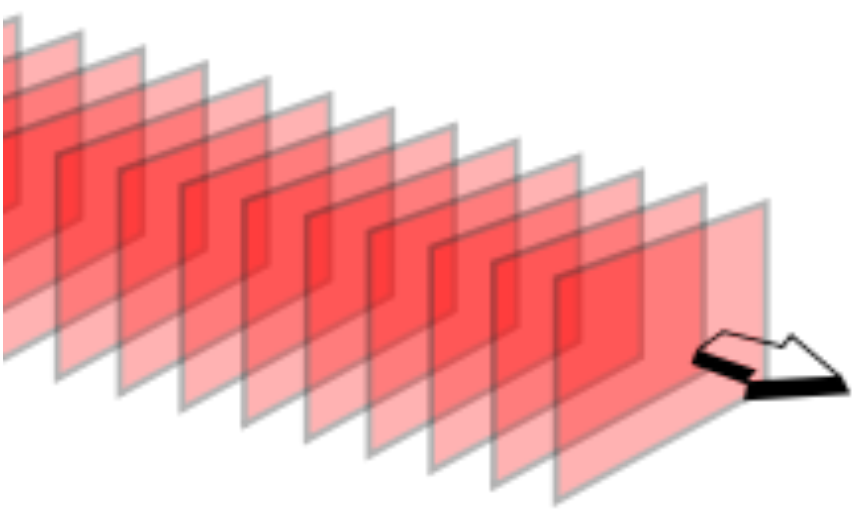
\includegraphics[width=0.3\linewidth]{pic/frontondesplan.png}
                \item Ondes Spherique : front d'ondes sont des sphere \\ 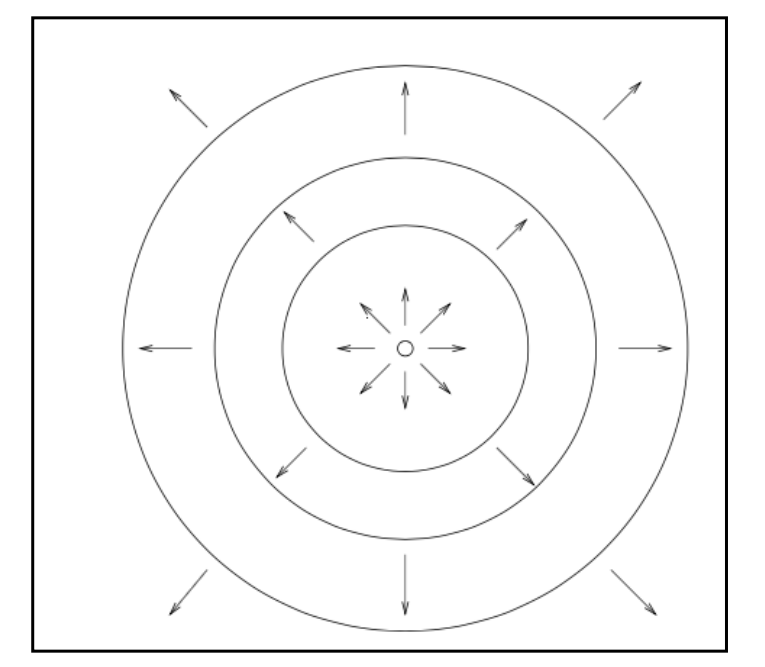
\includegraphics[width=0.3\linewidth]{pic/frontondessphere.png}
            \end{itemize}
        \section{Modelisation d ondes transversales sur une corde vibrant}
            On considere une corde homogene de section constant , de longueur fixe, de mass lineique fixe et inextensible
            $\alpha(x,t)<<1 \implies(\cos(\alpha) \cong 1 ,\sin(\alpha)\cong \alpha , \tan(\alpha)\cong \alpha)$\\
            

            \begin{center}
                \begin{minipage}{0,3\linewidth}
                    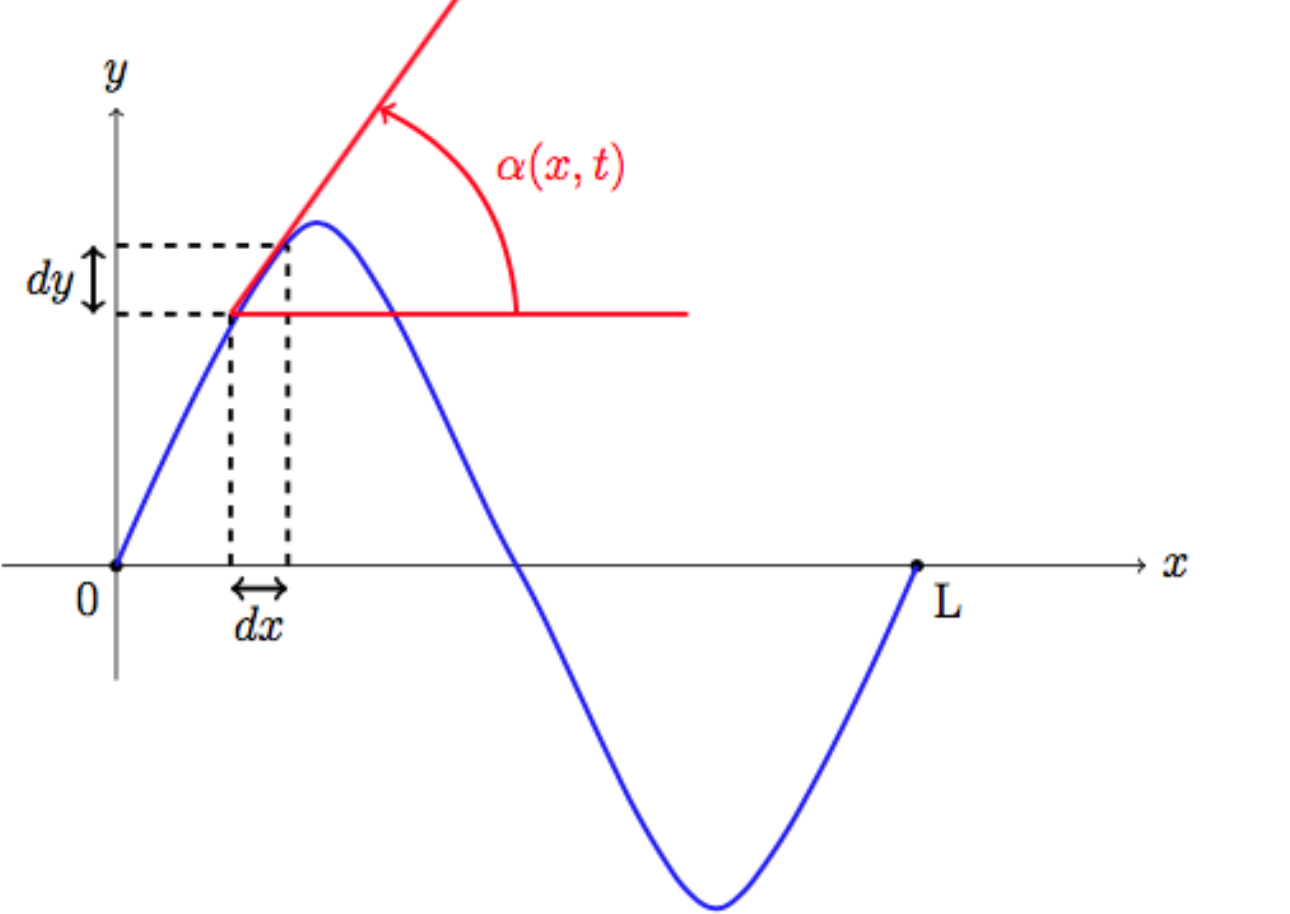
\includegraphics[width=\linewidth]{pic/modelisationdondescordevibrant.png}
                \end{minipage}
                \begin{minipage}{0,59\linewidth}
                    a un $dx$ il corspond une variation $dy$ , $dy =y(x+dx,t)-y(x,t)$ \\ avec $y(x+dx,t) = $\\$ y(x,t)+\underbrace{\frac{\partial y(x,t)}{\partial x}dx}_{\text{term de premier ordre}} + \underbrace{\ldots}_{\text{terms d order superieur}}$
                \end{minipage}
            \end{center}
            alors \begin{itemize}
                \item $dy =\frac{\partial y(x,t)}{\partial x}dx $
                \item $\tan(\alpha) = \frac{dy}{dx}=\frac{\partial y}{\partial x}$
                \item $ |\alpha| << 1 \implies |\frac{\partial y}{\partial x}|<<1 $
            \end{itemize}
        \section{Equation d almbert}
            \begin{center}
                \begin{minipage}{0,49\linewidth}
                    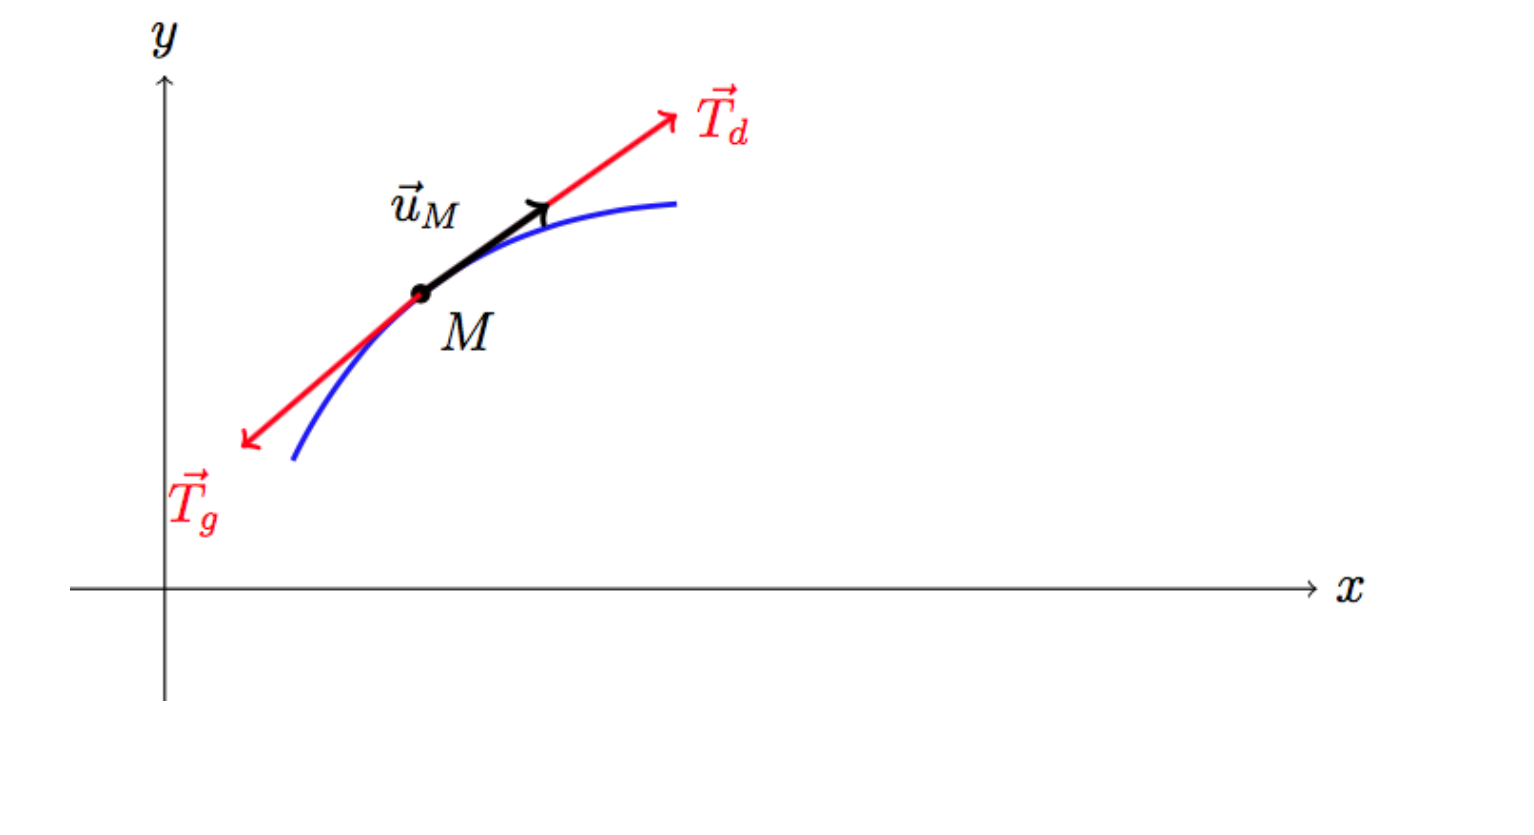
\includegraphics[width=\linewidth]{pic/tension.png}
                \end{minipage}
                \begin{minipage}{0,49\linewidth}
                    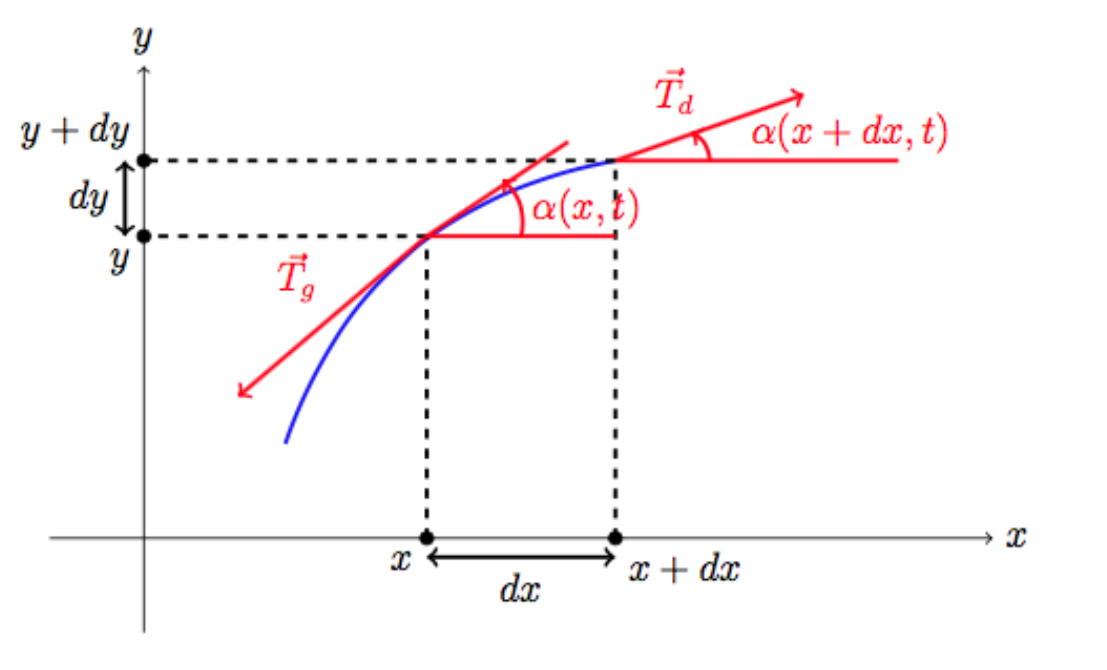
\includegraphics[width=\linewidth]{pic/tension2.png}
                \end{minipage}
            \end{center}
            l element de corde entre $x$ et $x+dx$ est $dl$ , $dl=\sqrt{dx^2+dy^2}=dx[1+\left( \frac{\partial y}{\partial x } \right)^2 ]^{\frac{1}{2}}$ \\ 
            \boxed{\frac{dy}{dx} = \frac{\partial y}{\partial x}} pour $|\frac{\partial y}{\partial x}|<<1$\\
            \underline{Principe dynamique :} $m\vv{a} = \vv{T_d}+\vv{T_g}$ avec $m=\mu dx$ ($\mu$ est la masse lineique) \\ 
            on a $\begin{cases}
                \vv{a_x} = \vv{0} & (\text{transversal}) \\
                \vv{a_y} = \frac{\partial y^2}{\partial t^2}\vv{u_y}=\vv{a}
            \end{cases}$ \\
            \begin{itemize}
                \item Projection sur $\vv{u_x} \implies 0 =T(x+dx,t)\cos(\alpha(x+dx,t)) - T(x,t)\cos(\alpha(x,t))$ \\
                    $\implies 0 = T(x+dx,t)-T(x,t) = \frac{\partial T}{\partial x}dx \implies$\boxed{\frac{\partial T}{\partial x}dx = 0} \\
                    $\implies$ la Tension est uniform le long du corde et ne depend que du temp :$T(t)=T_0$
                \item Projection sur $\vv{u_y} \implies \mu dx \frac{\partial^2y}{\partial t^2} = T_0\sin(\alpha(x+dx,t))-T_0\sin(\alpha(x,t))$\\
                    $\implies \mu dx \frac{\partial^2y}{\partial t^2} = T_0[\alpha(x+dx,t)-\alpha(x,t)] = T_0\frac{\partial \alpha}{\partial x}dx$ \\
                    avec $\tan(\alpha) \cong \alpha = \frac{\partial y}{\partial x} \implies $\boxed{\mu \frac{\partial^2y}{\partial t^2} =T_0\frac{\partial^2y}{\partial x^2}} 
            \end{itemize}
            \begin{center}
                \boxed{\frac{\partial^2 y}{\partial t^2} -\frac{T_0}{\mu}\frac{\partial^2 y}{\partial x^2} = 0 } c est lequation d'almbert
            \end{center}
            \subsection{Equation d almebert a 3D}
                $$ \frac{\partial^2 \psi }{\partial t^2} - c^2\Delta\psi =0 $$
                $\psi (x,y,z,t) = \psi(\vv{r},t)$
                \begin{itemize}
                    \item $\psi :$ un grandeur scalair ou vectoriel 
                    \item $ \Delta : $ operateur laplacien
                    \item $ c :$celerite 
                    \item Pas de phenomen dissipatif (pas de perd d energie)
                \end{itemize}
                \underline{Note}: dans le cas d'ondes transversal le long d'une corde vibrant $c = \sqrt{\frac{T}{\mu}}$
            \subsection{Solution de lequation d alembert (onde progressives)}
                $ \psi = \psi(x,t) \implies \frac{\partial^2 \psi }{\partial t^2}-c^2\frac{\partial^2 \psi }{\partial x^2} =0$ la solution general peut toujours secrire sous la form 
                $$  \psi(x,t) = f(t-\frac{x}{c}+g(t+\frac{x}{c })) $$
                Deux fonction $f(u)$ et $g(v)$ , chacune a une seule variable spatio-temporelle u ou v $\begin{cases}
                    f(u) & u = t-\frac{x}{c} \\ 
                    g(v) & v = t+\frac{x}{c}
                \end{cases}$\\
                \underline{Cas de $\psi_+ (f(u))$} \\
                    $$ \frac{\partial^2 \psi}{\partial t^2}-c^2 \frac{\partial^2\psi}{\partial x^2}=0 $$
                    \begin{itemize}
                        \item Chercher $\frac{\partial^2 \psi}{\partial t^2}$
                            $\frac{\partial \psi}{\partial t} = \frac{\partial \psi}{\partial u}\times\frac{\partial u}{\partial t}=\frac{\partial f}{\partial u}\times 1=f^{'}(u)\\
                             \implies \frac{\partial^2 \psi}{\partial t^2}=\frac{\partial}{\partial t}\left( \frac{\partial\psi}{\partial t} \right)=\frac{\partial}{\partial u}\underbrace{\left( \frac{\partial \psi}{\partial t} \right)}_{f^{'}(u)}\times\underbrace{\frac{\partial u}{\partial t}}_{1} \implies $
                             \boxed{\frac{\partial^2\psi}{\partial t^2} = f^{''}(u) }
                        \item Chercher $\frac{\partial^2\psi}{\partial x^2}$ \\
                            $\frac{\partial\psi}{\partial x}  = \frac{\partial \psi}{\partial u}\frac{\partial u}{\partial x} = \frac{\partial f}{\partial u}\times\frac{-1}{c}=\frac{-1}{c}f^{'}(u)$\\
                            $\implies \frac{\partial^2 \psi}{\partial x^2}=\frac{\partial}{\partial x}\left( \frac{\partial\psi}{\partial x} \right)=\underbrace{\frac{\partial}{\partial u}\left( \frac{\partial \psi}{\partial x} \right)}_{\frac{-1}{c}f^{'}(u)}\times\underbrace{\frac{\partial u}{\partial x}}_{\frac{-1}{c}}$
                            $\implies  $\boxed{\frac{\partial^2 \psi}{\partial x^2}=\frac{1}{c^2}f^{''}(u)}
                        \item  Remplacer $\frac{\partial^2\psi}{\partial x^2}$ et $\frac{\partial^2\psi}{\partial t^2}$ dans lequation $\implies f^{''}(u)-c^2\times\frac{1}{c^2}f^{'}(u) = 0$ \underline{VERIFIER}
                    \end{itemize}
                \underline{Cas de $\psi_-(g(v))$}\\ 
                meme methode que $\psi_+$
                \begin{center} 
                    \underline{RESUME} \\
                    \boxed{
                        \begin{cases}
                            \psi(x,t) = f(t-\frac{x}{c}) & x \nearrow \\
                            \psi(x,t) = f(t+\frac{x}{c}) & x \searrow  \\
                        \end{cases}
                    }
                \end{center}
        \section{Onde progressive}
            \subsection{Definition}
                Une onde qui se propage dans une direction reperees par un vecteur unitair $\vv{u}$ ,sans se deformer a la celerite $c$
            \subsection{harmonique}
                Une onde progressive est dite harmonique si sa dependence en temps est sinusoidale \\
                $$  \psi = a\cos(wt-kx+\phi_0)  $$ 
                pour que $\psi$ satisfe lequation d alembert \begin{itemize}
                    \item $w^2 = c^2k^2$
                    \item $k = \frac{w}{c}$
                \end{itemize}
                \underline{Preuve} \\
                $\frac{\partial^2 \psi}{\partial t^2} = -aw^2\cos(wt-kx+\psi_0)$\\
                $\frac{\partial^2 \psi}{\partial x^2} = -ak^2\cos(wt-kx+\psi_0)$\\
                $\frac{\partial^2 \psi}{\partial t^2} = c^2\frac{\partial^2\psi}{\partial x^2}$(dapres lequation d alembert) \\
                Donc , $\psi$ satisfait lequation de d'almbert pour $w^2=c^2k^2$ et $k=\frac{2}{c}$ avec $c > 0$\\
                $\begin{cases}
                    w : &\text{pulsation temporelle de londe }(T=\frac{2\pi}{w}) \\
                    k : &\text{pulsation spatiale de londe }(\lambda=\frac{2\pi}{k}) \\
                \end{cases}$
            \subsection{Phase instantanee}
                $\phi = wt - \vv{k}.\vv{r} + \phi_0$\\
                \underline{Surface d'onde}:Lieu de points de l'espace tel que à $t_0$ donné, la phase instantanée de l'onde est constante: $ \phi(m,t_0) = \phi_0 $ (surface équiphase ou isophase)\\
                \underline{Onde plane} :dont les surfaces d'onde sont des plans et dont l'amplitude est constante sur de tels plans\\
            \subsection{Vitesse de phase}
                \begin{itemize}
                    \item Soit $\psi(x,t) = a\cos(\phi(x,t))$ avec $\phi(x,t) = wt-kx+\phi_0$ 
                    \item Plan d'onde : $\phi(x,t) = \phi_0$ a $(x,t)$
                    \item a $t^{'} > t $,abscisse du plan est $x^{'}=x+l$ , $\phi(x{'},t^{'}) = \phi_0$
                    \item la valeur de vitesse de phase $v_\phi$ ? \\
                    $\Phi\left(x^{\prime}, t^{\prime}\right)=\Phi\left(x+l, t+\frac{l}{v_{\phi}}\right)=\Phi(x, t)=\Phi_{0}$\\
                    $w\left(t+\frac{l}{v_{\phi}}\right)-k(x+l)+\phi_{0}=w t-k x+\phi_{0}$\\
                    $w t-k x+\phi_{0}+\left(w \cdot \frac{l}{v_{\phi}}-k . l\right)=w t-k x+\phi_{0}$\\
                    $\frac{2}{v_\phi} = k \implies v_\phi = \frac{w}{k} = c$( car satisfait lequation de d'alembert) \\
                    Le milieu transmet l'onde a la meme vitesse pour tout sa frequence $w \implies$ milieu non dispersif
                \end{itemize}
        \section{Representation complexe}   
            $ \psi(x,t) = a\cos(wt-kx+\phi_0) \implies\underline{\psi}(x,t)=\psi_0e^{i(wt-kx)} \;, \psi_0 =ae^{i\psi_0} $ \\
            Tell que $\psi(x,t)=\mathfrak{R}(\underline{\psi}(x,t)) $
        \section{Solution d equation d almbert en termes d'ondes stationnaires}
            C est tout solution d equation d Almbert sous la form \\ $\psi(x,t)=F(x)G(t)$ 
            avec $\begin{cases}
                G(t)=G_0\cos(wt+\phi_G)\\
                F(x)=F_0\cos(\frac{w}{c}x+\phi_F)
            \end{cases}$ \\
            \begin{center}
                \boxed{\psi =\psi_0\cos(wt+\phi_G).\cos(\frac{w}{c}x+\phi_F)}
            \end{center}
            \begin{center}
                \begin{minipage}{0,49\linewidth}
                    \begin{itemize}
                        \item il ny a plus de propagation 
                        \item les point ou $\psi =0$ sont des noeud
                        \item les point ou $\psi $ est maximal sont des voentres
                    \end{itemize}
                \end{minipage}
                \begin{minipage}{0,49\linewidth}
                    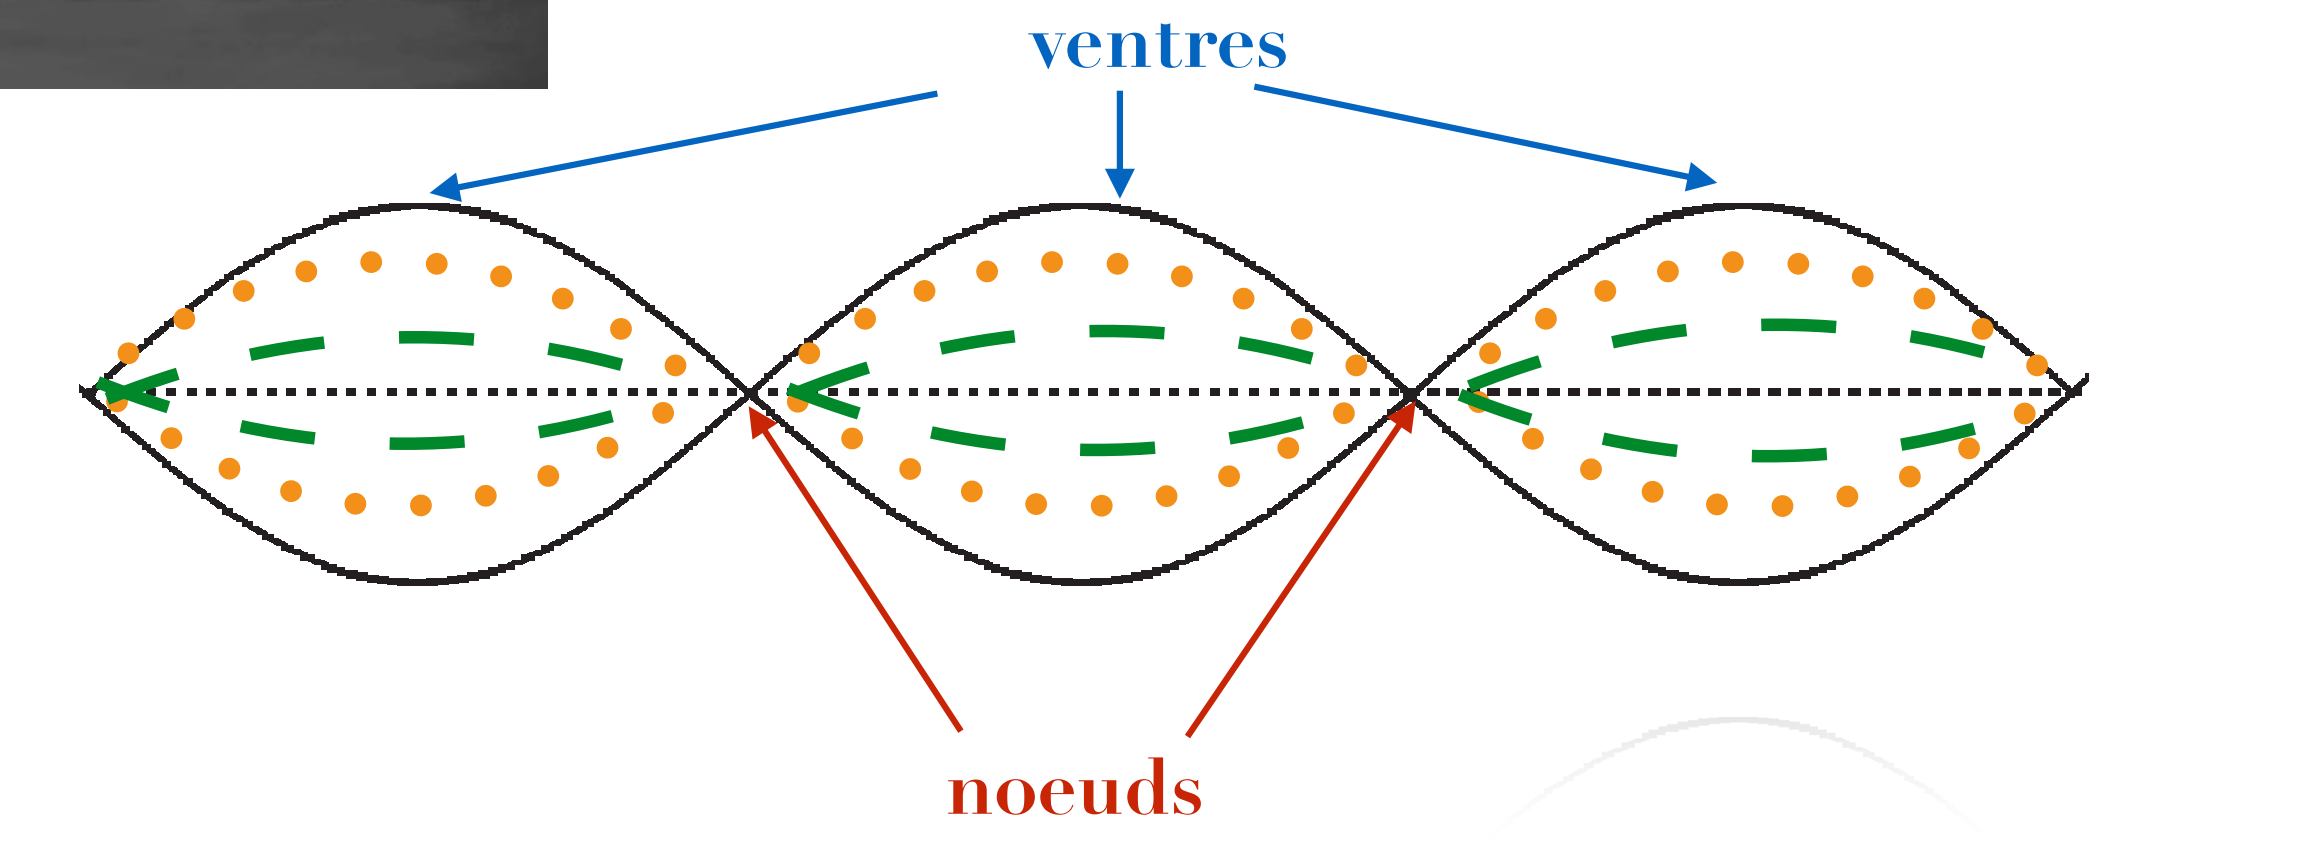
\includegraphics[width=\linewidth]{pic/stationair.png}
                \end{minipage}
            \end{center}
            $\psi  $ elle peut ecrire sous la form : 
            \begin{center}
                \boxed{\frac{\psi_0}{2} (\cos(\underbrace{wt+kx}_{x \searrow}+\phi_G+\phi_F) +\cos(\underbrace{wt-kx}_{x\nearrow }+\phi_G+\phi_F)) }
            \end{center}
            alors on peut dire que l onde stationair est une superposition de deux ondes progressives harmonique de meme amplitude et de sense oppose
            \subsection*{Note bien}
                En peut ecrice le fonction du corde vibrant sous la form d'onde stationair 
                \[ y(x,t) = Y \sin(kx)\sin(wt) \]
                avec \begin{itemize}
                    \item des condition au limite ou les borne du corde a un $ y=0 $
                    \item $k = \frac{n\pi}{L}$
                    \item $ w = \frac{n\pi c }{L} = \frac{n\pi }{L}\sqrt{\frac{T}{\mu}} $ 
                    \item $ w = 2\pi f $
                    \item $ n $ : nombre des ventre 
                    \item  $ c $ : celerite $ c=\sqrt{\frac{T}{\mu}} $
                    \item $ L $ : longueur du corde
                    \item $ T  $ : Tension du corde 
                    \item $ \mu $ : mass lineique
                \end{itemize}
                La notion \underline{corde sans raideur} $ \implies $ pas d'elasticite est alors lea sele force a prendre en compte est celle de tension \\
                car la raideur traduit la capacite de la corde a se deforme \\ 
                La notion \underline{des petit mouvement } $ \implies $ les deplacements de la corde sont petits $ \implies $ toutes les variable d'etat et leurs derive sont des terme de premier ordre \\ 

                    
    \chapter{Ondes sonores dans les fluids}
        \section{Definiton}
            \begin{itemize}
                \item Une onde sonore est une onde logitudinales de surpression (variation de la pression par rapport a letat d equilibre)
                \item se propage dans un milieu materiel (l elasticite du milieux qui permet la propagation)
            \end{itemize}
        \section{Propagation d une onde sonore}
            \begin{itemize}
                \item le fluide est decrit par \\
                    \begin{itemize}
                        \item Champ de vitesse $\vv{v}(M,t)$ (vitesse de la particule de fluide situe en $M$ a l instant $t$)
                        \item Champ de pression $P(M,t)$
                        \item Champ de mass volumique $\mu (M,t) $
                    \end{itemize}
                \item Dans le cas d absence d'onde sonore (fluide au repos) \\
                    Champ uniform $\begin{cases}
                        \vv{v}(x,t)=\vv{0} \\
                        P(M,t)=P_0 \\
                        \mu(M,t)=\mu_0
                    \end{cases}$
                \item En presence de londe sonore \\
                    $\begin{cases}
                        \vv{v}(x,t)=\vv{v_1}(M,t) \\
                        P(M,t)=P_0+P_1(M,t) \\
                        \mu(M,t)=\mu_0+\mu_1(M,t)
                    \end{cases}$
            \end{itemize}
        \section{Approximation acoustique}
            Concernent les champs qui caracterise l onde sonore 
            \begin{itemize}
                \item les champ sont des infiniment petite du meme order, ainsi que leurs derivees spatiales et temporelles
                \item leur moyenne temporelle est nulle \\
                $<p_{1}(M, t)>=0 ; \quad<\mu_{1}(M, t)>=0 \quad$ et $<\vec{v}_{1}(M, t)>=\overrightarrow{0}$
            \end{itemize}
        \section{Equation d ondes sonore}
            l equation des ondes sonores est etablie a partir des equation d ecrivant l evolution du fluide :
                \begin{itemize}
                    \item  1 Equation d Euler 
                    \item  2 Conservatoin de la matiere 
                    \item  3 Evolution thermodynamique
                \end{itemize}
            \subsection{Equation d Euler}
                lequation d euler secrit , en negligent la pesanteur : \\ 
                $(\mu_0 + \mu(M,t))\left[\frac{\partial \vv{v_1}}{\partial t}+(\vv{v_1}(M,t).\vv{grad})\vv{v_1}(M,t) \right] = -\vv{grad}P(M,t)$ \\
                $\vv{grad}P(M,t) = \vv{grad}(P_0+P_1)=\vv{grad} P_1$\\
                les termes $\mu_1\frac{\partial\vv{v_1}}{\partial t},(\vv{v_1}\vv{grad})\vv{v_1}$ sont d order 2 \\
                alor par Approximation acoustique \boxed{\mu_0 \frac{\partial\vv{v_1}}{\partial t}=-\vv{grad}P_1(M,t)}
            \subsection{Conservation de la matiere}
                l equation de la conservatoni de la matiere \\
                $\frac{\partial \mu_1}{\partial t}+\operatorname{div}(\mu \cdot \vec{v})=0 $ avec $\quad (\mu(M, t)=\mu_{0}+\mu_{1}(M, t))$\\
                $\frac{\partial \mu_{1}}{\partial t}+\operatorname{div}\left(\left(\mu_{1}+\mu_{0}\right) \vec{v}\right)=0$\\
                $\frac{\partial \mu_{1}}{\partial t}+\mu_{0} \operatorname{div} \vec{v}_{1}+\underbrace{\operatorname{div}\left(\mu_{1} \vec{v}_{1}\right)}_{\text{terme d order 2}}=0 \implies$
                \boxed{\frac{\partial \mu_{1}(M, t)}{\partial t}+\mu_{0} \operatorname{div} \vec{v}_{1}(M, t)=0}
            \pagebreak
            \subsection{Adiabatisme}
                \begin{itemize}
                    \item Une transformation est appelee adaibatique lorsque le systeme n'echange pas de chaleur avex le milieu exterieur 
                    \item Une transformation reversible (quantite) est une transformation ou aucune entropie est produit 
                    \item Adiabatique + reversible $\implies$ isentropique(meme entropie $S$)\\
                        Cela restreint l amplitude de surpression (pas de perd d energie)
                    \item Coefficient de compresibilite adiabatique de fluide $\x_s = \frac{1}{\mu}(\frac{\partial \mu}{\partial p})$
                    \item $d\mu$ et $dp$ sont reliees par \\
                        \boxed{d\mu = \left( \frac{\partial \mu}{\partial P} \right)dp = \mu\x_sdP}
                    \item d'autre part , les variations des champs $\mu$ et $P$ s ecrivent : \\
                        $d\mu = \frac{\partial\mu}{\partial t}dt + \frac{\partial \mu}{\partial x}dx + \frac{\partial \mu}{\partial y}dy + \frac{\partial \mu}{\partial z}dz = \frac{\partial\mu}{\partial t}dt + \left( \frac{\partial \mu}{\partial x}\frac{dx}{dt} + \frac{\partial \mu}{\partial y}\frac{dy}{dt} + \frac{\partial \mu}{\partial z}\frac{dz}{dt}  \right) \times dt$ \\
                        de meme $dP=\left( \frac{\partial P}{\partial t} +\vv{v}.\vv{grad}{} \right)dt$ \\
                        dans le cadre de lapproximation acoustique on neglige les termes d order 2 \\ $\implies$ \boxed{d\mu=\frac{\partial \mu_1}{\partial t}dt} et\boxed{dP=\frac{\partial P_1}{\partial t}dt}
                \end{itemize}
                alors \begin{align*}
                    d\mu &= \mu\x_s(\frac{\partial P_1}{\partial t})dt \\
                    (\frac{\partial\mu_1}{\partial t}) &= \mu\x_s(\frac{\partial P_1}{\partial t})\\
                    &=[\mu_0 +\mu_1]\x_s\left( \frac{\partial P_1}{\partial t} \right) \; \; \; (\mu_1\frac{\partial P_1}{\partial t}\text{est d ordre 2}) \\
                    &=\mu_0\x_s\frac{\partial P_1}{\partial t}
                \end{align*}\\
                \begin{center}
                     \boxed{\mu_1(M,t) = \mu_0\x_sP_1(M,t)}
                \end{center}
                \pagebreak
                \underline{Synthese}
                \begin{itemize}
                    \item  1 Equation d Euler : \boxed{\mu_0 \frac{\partial\vv{v_1}}{\partial t}=-\vv{grad}P_1(M,t)} (1)
                    \item  2 Conservatoin de la matiere : \boxed{\frac{\partial \mu_{1}(M, t)}{\partial t}+\mu_{0} \operatorname{div} \vec{v}_{1}(M, t)=0} (2)
                    \item  3 Evolution thermodynamique : \boxed{\mu_1(M,t) = \mu_0\x_sP_1(M,t)} (3)
                \end{itemize}
                \underline{Suit de calcule}\\
                    Dapres $(1) \; \mu_0 \frac{\partial\vv{v_1}}{\partial t}=-\vv{grad}P_1(M,t)$ \\
                    $\implies div(\vv{grad}P_1(M,t)) = -\mu_0div\left( \frac{\partial \vv{v_1}}{\partial t} \right) = -\mu_0\frac{\partial}{\partial t}(div\vv{v_1})$ \\
                    Dapres $ (2) \; \mu_{0} \operatorname{div} \vec{v}_{1}(M, t) =-\frac{\partial \mu_{1}(M, t)}{\partial t} $\\
                    $\frac{\partial (2)}{\partial t} \implies \mu_{0} \frac{\partial}{\partial t}\operatorname{div} \vec{v}_{1}(M, t) =-\frac{\partial^2 \mu_{1}(M, t)}{\partial t^2} $\\
                    En utilisant (1) $\implies div(\vv{grad}P_1(M,t)) = -\mu_0\frac{\partial}{\partial t}(div\vv{v_1})=\frac{\partial^2 \mu_{1}(M, t)}{\partial t^2} $ \\
                    En utilisant (3)$\mu_1(M,t) = \mu_0\x_sP_1(M,t) \implies div(\vv{grad}P_1(M,t)) = -\mu_0\frac{\partial}{\partial t}(div\vv{v_1})=\frac{\partial^2 \mu_{1}(M, t)}{\partial t^2} = \mu_0\x_s\frac{\partial^2 P_1(M,t)}{\partial t^2}$\\
                    on a l operateur laplacien est definie par : $\Delta = div(\vv{grad}) alors $
                    \begin{center}
                        \boxed{\frac{\partial^2P_1(M,t)}{\partial t^2}-\frac{1}{\mu_0\x_s}\Delta P_1(M,t)=0} (l equation de dalembert pour la surpression) \\
                        la celerite est donnees par : $c=\frac{1}{\sqrt{\mu_0\x_s}}$
                        
                    \end{center}
        \section{Celerite des ondes dans un gaz parfait }
            \begin{itemize}
                \item ona une evolution isentropique $\implies PV^\gamma = cte$\\
                    $\implies d(PV^\gamma) =\frac{\partial (PV^\gamma)}{\partial v}dv + \frac{\partial (PV^\gamma)}{\partial P}dp =0 $  \\
                    $\implies V^\gamma \times P (\gamma\frac{dV}{V}+\frac{dP}{P}) = 0 \implies \frac{dP}{P} + \gamma\frac{dV}{V}=0$ \\
                    alors en deduit l'expression du coefficient de compressibilite \\
                     on a $\x_s=\frac{-1}{V}\left( \frac{\partial V}{\partial P}\right) \implies$  \boxed{\x_s=\frac{1}{\gamma P} }
                \item la celerite a lordre le plus bas non nul $c = \frac{1}{\sqrt{\mu_0\x_s}} =\sqrt{\frac{\gamma P}{\mu_0}}=\sqrt{\frac{\gamma P_0}{\mu_0}}$ ici l order zero : $P=P_0$
                \item l equation d etat des gaz parfaits : $P = \frac{nRT}{V}$ avec $\mu V = masse = nM$
            \end{itemize}
            \begin{center}
                \boxed{c=\sqrt{\frac{\gamma R T_0}{M}}}
            \end{center}
        \section{Solutin de l'equation de d almebert}
            la solution : \\
                $p_1(M,t) = p_0\cos(wt-\vv{k}\vv{r}+\phi) , \; \vv{k} = k\vv{u}=\frac{2\pi}{\lambda}\vv{u} , \; w=c.k $ \\
            en notation complexe :
                $\underline{p_1} (M,t)= \underline{p_0}e^{i(wt-\vv{k}\vv{r})}$
        \section{les equation de l'acoustique lineaire en notation complexe}
            $\begin{cases}
                \underline{p_1} = \underline{p_0}e^{i(wt-\vv{k}\vv{r})}\\
                \underline{v_1} = \underline{v_0}e^{i(wt-\vv{k}\vv{r})}\\
                \underline{\mu_1} = \underline{\mu_0}e^{i(wt-\vv{k}\vv{r})}
            \end{cases}$\\
            \begin{itemize}
                \item \underline{Equation d'Euler}\\
                    $\mu_0w\underline{\vv{v_1}}(M,t) = \underline{p_1}(M,t)\vv{k}$ 
                \item \underline{Conservation de la masse}\\
                    $w\underline{mu_1}(M,t) = \mu\vv{k}.\underline{\vv{v_1}}(M,t)$
                \item \underline{Adiabaticite}\\
                    $\underline{\mu_1}(M,t) = \mu_0\x_s\underline{p_1}(M,t)$
            \end{itemize}
        \section{Impedance acoustique}
            \begin{itemize}
                \item  on a $\mu_0w\underline{v_1}(M,t)\vv{u} = \underline{p_1}(M,t)k\vv{u} $
                \item En utilisant $w=ck$ \\
                    $\mu_0 c\underline{v_1}(M,t) = \underline{p_1}(M,t) \implies \underline{p_1}(M,t) = \sqrt{\frac{\mu_0}{\x_s}}\underline{v_1}$
                \item en prenant la partie relle \boxed{p_1(M,t) = \mu_0cv_1=\sqrt{\frac{\mu_0}{\x_s}}v_1}\\
                    La surpression et la vitesse sont en phase , Leur rapport ne depend que des caracteristique du milieu , il definit l'impedance acoustique du milieu 
                \item Impedance acoustique :$Z_a =\frac{p_1}{v_1}=\mu_0c=\sqrt{\frac{\mu_0}{\x_s}} $
                    l impedance acoustique caracterise la resistance du milieu au passage de cette onde
            \end{itemize}
            \underline{Note}Pour une onde plane progressive harmonique se propageant dans les sens oppose $-\vv{u}$, limpedance acoustique est : $Z_a = -\sqrt{\frac{\mu_0}{\x_s}}$
        \section{Aspects energetiques}
            l'onde sonore est caracterisee par : \\
                \begin{itemize}
                    \item \underline{Onde de vitesse } (deplacement de particules)$ \implies $(energie cinetique) 
                    \item \underline{Onde de pression} ( compression/dilatation des particules) $\implies$ ( energie potentielle)    
                \end{itemize}
            \subsection{Expression locale du bilan d'energie}
                $$ \frac{\partial e(M,t)}{\partial t} + div\vv{\Pi}(M,t) = 0  $$ 
                $\vv{\Pi} :$ vecteur densite de courant energetique , $\vv{\Pi} = P_1(M,t)\vv{v_1}(M,t)$ \\
                la norme  $|| \vv{\Pi}(M,t) || $ e exprime en $w/m^2$ \\
                l expression devient \boxed{\frac{\partial e(M,t)}{\partial t} + div(p_1\vv{v_1}) = 0} avec $div(p_1\vv{v_1})=p_1div(\vv{v_1})+\vv{v_1}\vv{grad}(p_1)$ \\
                D'apres l'equation d'euler :$\vv{grad}p_1(M,t)=-\mu_0\frac{\partial \vv{v_1}}{\partial t}$ \\
                D'apres les equations de conservation de masse et d'adiabaticite $\begin{cases}
                    \frac{\partial \mu_{1}(M, t)}{\partial t}+\mu_{0} \operatorname{div} \vec{v}_{1}(M, t)=0 \\
                    \mu_1(M,t) = \mu_0\x_sP_1(M,t)
                \end{cases}$
                $div\vv{v_1}(M,t)=-\x_s\frac{\partial p_1(M,t)}{\partial t}$ \\
                On remplace les valeurs de $div(\vv{v_1})$ et de $\vv{grad}(p_1)$ dans l equation :\\
                $\begin{aligned}
                    \operatorname{div}\left(p_{1} \vec{v}_{1}\right) &=p_{1} \operatorname{div}\left(\vec{v}_{1}\right)+\vec{v}_{1} \overrightarrow{\operatorname{grad}}\left(p_{1}\right) \\
                    &=-p_{1} \chi_{S} \frac{\partial p_{1}(M, t)}{\partial t}-\vec{v}_{1} \mu_{0} \frac{\partial \vec{v}_{1}}{\partial t}     \\
                    \implies\operatorname{div}\left(p_{1} \vec{v}_{1}\right)&=-\frac{\partial}{\partial t}\left(\frac{1}{2} \chi_{S} p_{1}^{2}+\frac{1}{2} \mu_{0} \vec{v}_{1}^{2}\right) \text{et on a }\frac{\partial e(M,t)}{\partial t} + div(p_1\vv{v_1}) = 0         
                \end{aligned}$\\
               Alors \begin{center}
                    Densite volumique d'energie : \boxed{e(M,t) = \underbrace{\frac{1}{2}\x_sp_1^2}_{\scriptsize\Centerstack{densite d'energie potentielle \\ emmagasinee par le fluide \\ sous l' effet des forces de pression}}+\underbrace{\frac{1}{2}\mu_0\vv{v_1^2}}_{\scriptsize\Centerstack{densite d'energie cinetique\\ du fluide}} }
               \end{center}
               \pagebreak
            \subsection{Cas d'une onde plan progressive harmonique selon la direction $\vec{u}$ }
               $p_1=\mu_0c\vv{v_1}=v_1\vv{u}$ \\
               la densite d'energie potentielle : $e_p =\frac{1}{2}\chi_sp_1^2=\frac{1}{2}\chi_s\mu_0^2c^2v_1^2 \underbrace{ = }_{c^2 = \frac{1}{\mu_0\chi_s}}\frac{1}{2}\mu_0v_1^2 = e_c$ \\
               la densite d'energie sonore est alors :$e=e_c+e_p=2e_c=\mu_0v_1^2=\chi_sp_1^2$ \\
               le vecteur densite de courant energetique : $\Pi = p_1\vv{v_1}=\mu_0cv_1^2\vv{u}=\frac{p_1^2}{\mu_0c}\vv{u}$
        \section{Intensite et niveau sonores}
            \begin{itemize}
                \item\underline{Intensite sonore } : represente la puissance moyenne transportee par l'onde par unite de surface et s'exprime en $W/m^2$ \\
            $$ I = \langle ||  \vv{\Pi}(M,t)  || \rangle  $$
            dans le cas d 'une onde plan progressive harmonique elle secrit : $I = \frac{\langle p_1^2(M,t) \rangle}{\mu_0c} $ \\ 
            avec $p_1(M,t) = p_{1m}cos(wt - \vv{k}.\vv{r}) \\ \implies\langle p_1^2(M,t) \rangle=\langle p_{1m}^2cos(wt - \vv{k}.\vv{r})^2 \rangle = \frac{1}{2} \langle p_{1m}^2(M,t) \rangle$ \\
            Alors $I = \frac{\langle p_{1m}^2(M,t) \rangle}{2\mu_0c}=\frac{\langle p_{1m}^2 \rangle}{2Z_a}$ ou $Z_a $ est l'impedance acoustique du milieu
                \item \underline{Niveau sonore} $I_{dB} = 10\log\frac{I}{I_0}$(decibel) ou Intensite de reference : $I_0 =10^{-12}W/m^2 $
            \end{itemize}      
        \section{Reflexion et transmission entre 2 milieux}
            \begin{center}
                \begin{minipage}{0.49\linewidth}
                    \begin{itemize}
                        \item Milieu (1) : $ x<0 $ mass volumique $\mu_{01}$ , celerite des ondes $c_1$ . L'impedance acoustique $Z_1 = \mu{01}c_1$
                        \item Milieu (2) : $ x>0 $ mass volumique $\mu_{02}$ , celerite des ondes $c_2$ . L'impedance acoustique $Z_2 = \mu{01}c_2$
                    \end{itemize}
                \end{minipage}
                \begin{minipage}{0.49\linewidth}
                    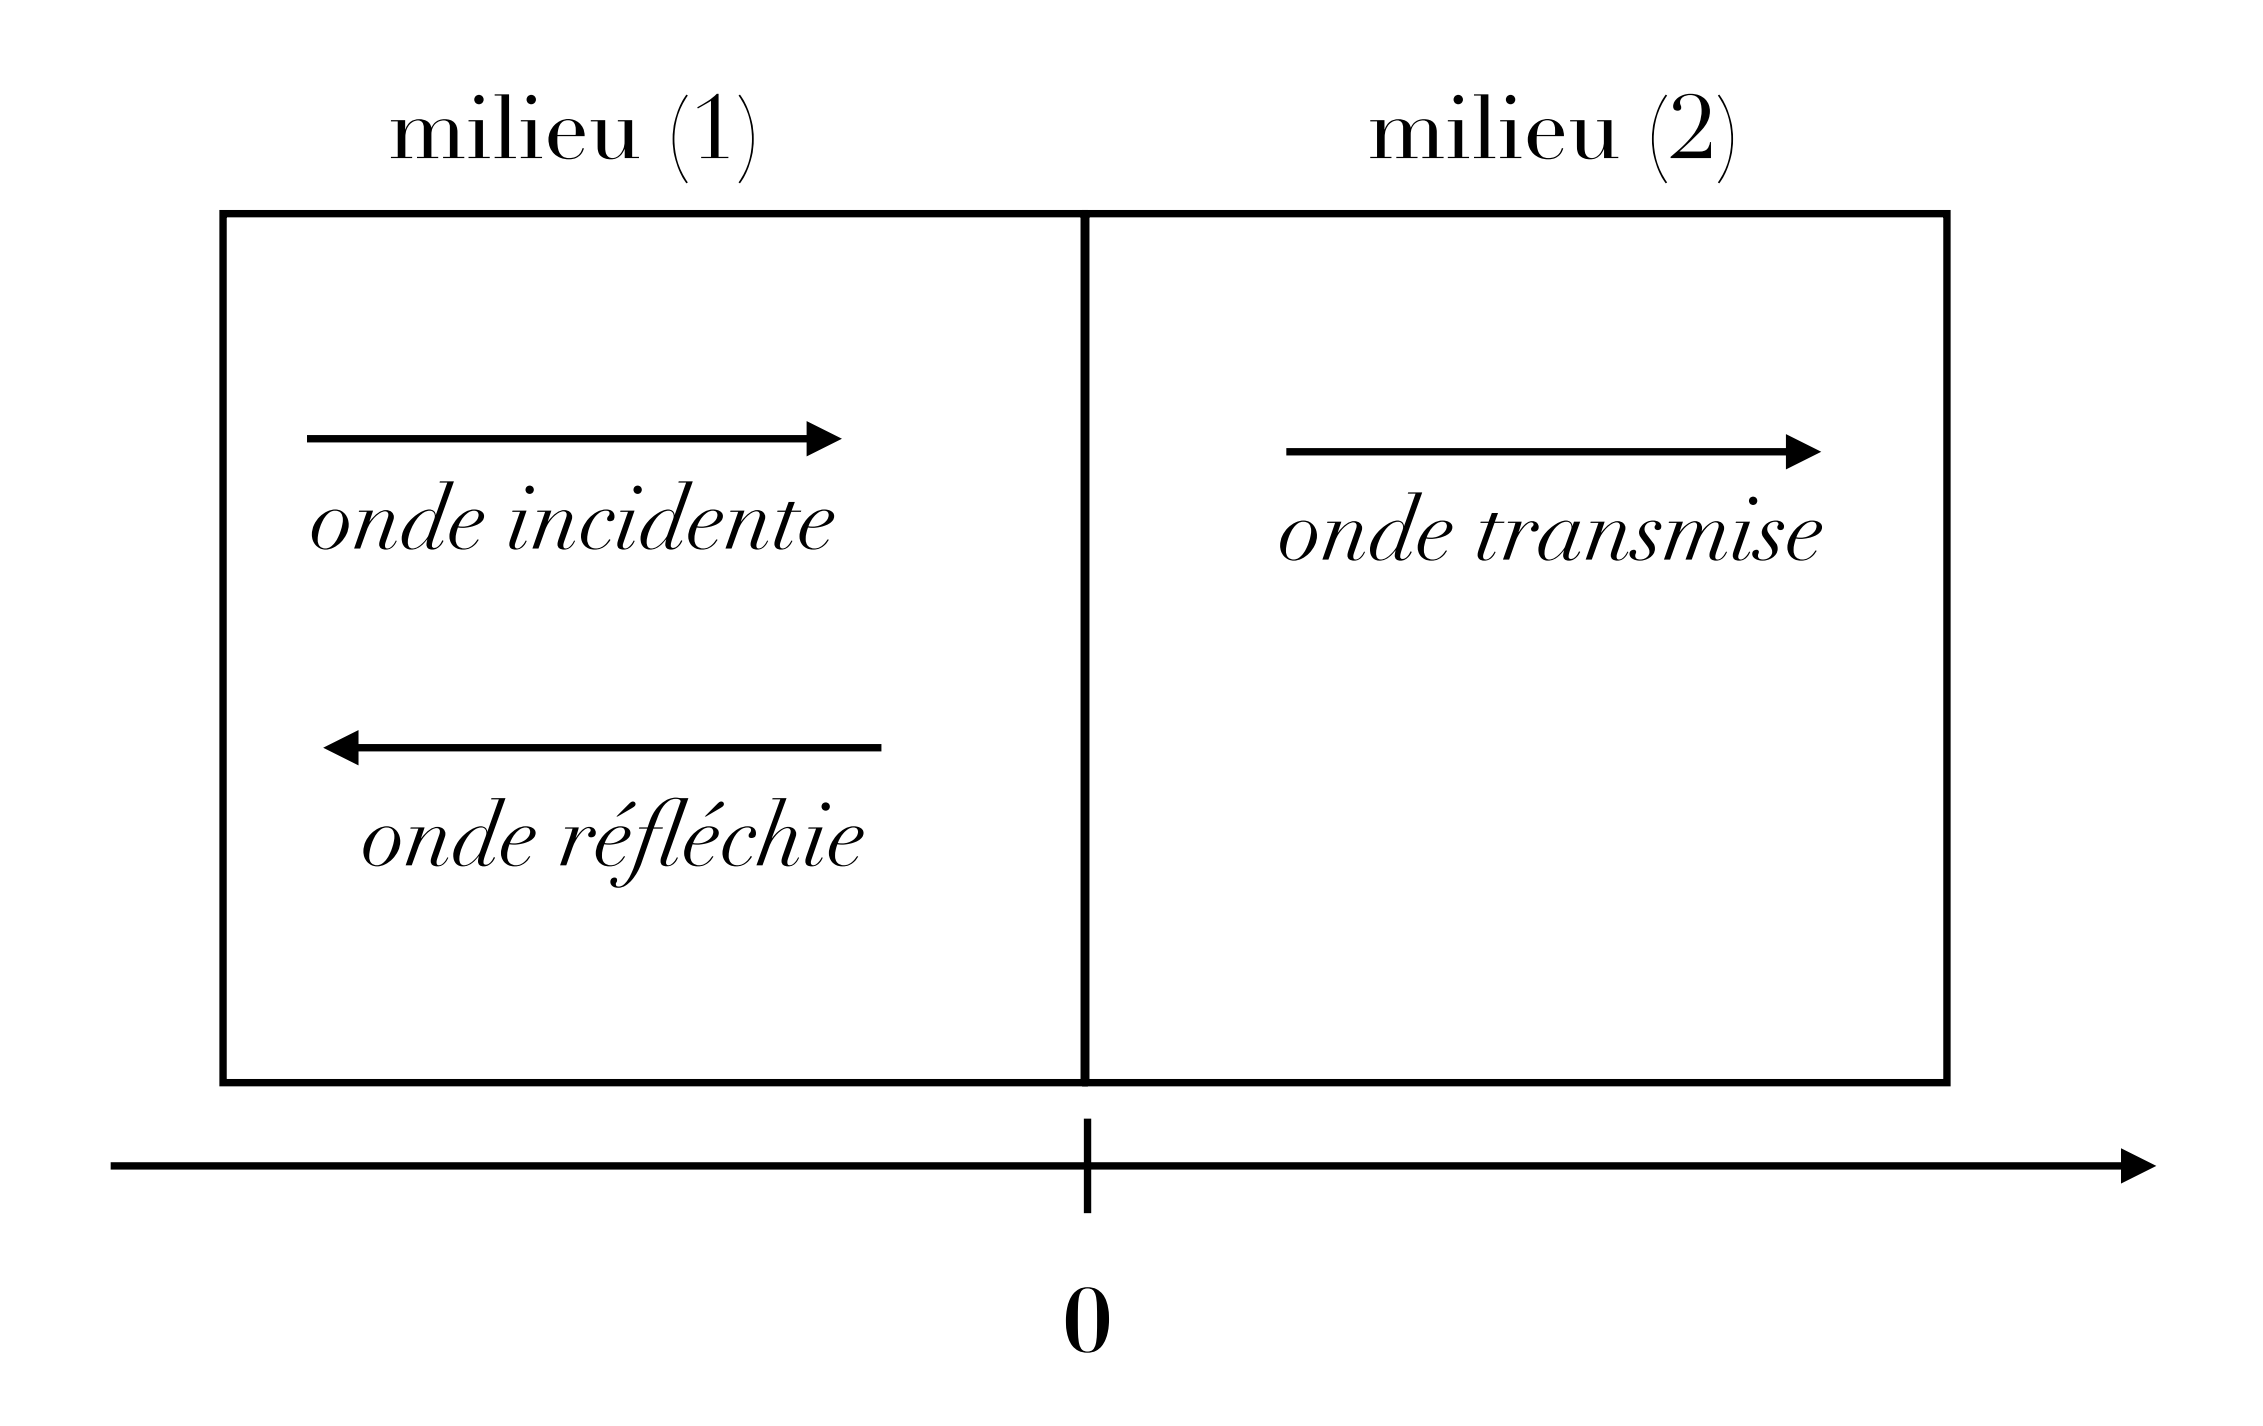
\includegraphics[width=\linewidth]{pic/reftran2milieu.png} 
                \end{minipage}
            \end{center}     
            \underline{Surpression et vitesse par rapport a l'ondes }
            \begin{itemize}
                \item Pour l'onde incidente
                    $p_i(x,t)=f(t-\frac{x}{c_1})$ et $v_i(x,t) = \frac{1}{Z_1}f(t-\frac{x}{c_1})$
                \item Pour l'onde reflechie
                    $p_r(x,t)=g(t+\frac{x}{c_1})$ et $v_r(x,t) = \frac{1}{Z_1}g(t+\frac{x}{c_1})$
                \item Pour l'onde transmise
                    $p_t(x,t)=h(t-\frac{x}{c_2})$ et $v_t(x,t) = \frac{1}{Z_2}h(t-\frac{x}{c_2})$
            \end{itemize}
            \underline{Note :}Puisque on a une 2 ondes dans le milieu 1 (incident et reflechie) alors il existe une \underline{superposition} \\ 
            \underline{Surpression et vitesse par rapport a la milieu}
            \begin{itemize}
                \item $ p(x,t)=\begin{cases}
                    f(t-\frac{x}{c_1})+g(t+\frac{x}{c_1}) & x<0 \\
                    h(t-\frac{x}{c_2}) & x>0 
                \end{cases}$
                \item $ v(x,t)=\begin{cases}
                    \frac{1}{Z_1}[f(t-\frac{x}{c_1})+g(t+\frac{x}{c_1})] & x<0 \\
                    \frac{1}{Z_2}h(t-\frac{x}{c_2}) & x>0 
                \end{cases}$
            \end{itemize}


            

\end{document}




